\documentclass[UTF-8,twoside,cs4size]{ctexart}
\usepackage{amsmath}
\usepackage{amssymb}
\usepackage{geometry}
\usepackage{setspace}
\usepackage{xeCJK}
\usepackage{ulem}
\usepackage{pstricks}
\usepackage{pstricks-add}
\usepackage{bm}
\usepackage{mathtools}
\usepackage{breqn}
\usepackage{mathrsfs}
\usepackage{esint}
\usepackage{textcomp}
\usepackage{upgreek}
\usepackage{pifont}
\usepackage{tikz}
\usepackage{circuitikz}
\usepackage{caption}

\geometry{a4paper,centering,top=0.75cm,bottom=2.54cm,left=2cm,right=2cm}
\pagestyle{plain}
\captionsetup{font=small}

\CTEXsetup[name={,.}]{section}
\CTEXsetup[format={\raggedright\bfseries\noindent\Large}]{section}
\CTEXsetup[format={\raggedright\bfseries\quad\large}]{subsection}

\setstretch{1.5}

\setCJKfamilyfont{boldsong}[AutoFakeBold = {2.17}]{SimSun}
\newcommand*{\boldsong}{\CJKfamily{boldsong}}
\DeclareMathOperator\dif{d\!}

\begin{document}
	\begin{flushright}
		\zihao{2}{分组号:3-07}
	\end{flushright}
	
	\noindent{\zihao{-2}\boldsong\bfseries 《\,\, 基\,\, 础\,\, 物\,\, 理\,\, 实\,\, 验\,\, 》\,\, 实\,\, 验\,\, 报\,\, 告\,\, }
	
	\noindent\textit{实验名称\uline{\quad\,\, 用示波器观测动态磁滞回线\,\,\,\qquad\qquad\qquad\qquad\qquad}指导教师\uline{\qquad\,\,\,高林青\,\,\,\qquad}}
	
	\noindent\textit{姓\qquad 名\uline{\,\,\, 桂庭辉\,\,\,}\,学号\uline{\,\,\,{\upshape2019K8009929019}\,\,\,}\,专\qquad 业\uline{\,\,\,计算机科学与技术\,\,\,}\,班级\uline{\,\,\,\upshape{03}\,\,\,}\,座号\uline{\,\,\,\upshape{6}\,\,\,}}
	
	\noindent\textit{实验日期\uline{\,\,{\upshape 2020}\,\,}年\uline{\,\,{\upshape 11}\,\,}月\uline{\,\,{\upshape04}\,\,}日\,\,实验地点\uline{\,\,\,教学楼{\upshape705}\,\,\,}调课/补课\uline{\,\,\,$ \square $是\,\,\,}成绩评定\uline{\,\,\,\quad\qquad\qquad}}
	
	\begin{table}[h]
		\centering
		\psset{linewidth=2pt}
		\begin{pspicture}(-1,-0.1)(1,0.1)
		\psline(-9,0)(9,0)
		\end{pspicture}
	\end{table}

	\section{实验目的}
	1.掌握利用示波器测量铁磁材料动态磁滞回线的方法;
	
	2.了解铁磁性材料的动态磁化特性;
	
	3.了解磁滞、磁滞回线和磁化曲线的概念,加深对饱和磁化强度、剩余磁化强度、矫顽力等物理量的理解。
	
	\section{实验器材}
	磁特性综合测量仪(包含正弦波信号源,待测样品及绕组,积分电路所用电阻和电容),双踪示波器,直流电源,电感,数字多用表。
	
	磁特性综合测量仪主要技术指标如下:
	
	(1)样品1:锰锌铁氧体,圆形罗兰环,磁滞损耗较小。平均磁路长度$ l=0.130\,\mathrm{m} $,铁芯实验样品截面积$ S=1.24\times10^{-4}\,\mathrm{m}^2 $,线圈匝数:$ N_1=N_2=N_3=150\,\text{匝} $。
	
	(2)样品2:EI型硅钢片,磁滞损耗较大。平均磁路长度$ l=0.075\,\mathrm m $,铁芯实验样品截面积$ S=1.20\times10^{-4}\,\mathrm m^2 $,线圈匝数:$ N_1=N_2=N_3=150\,\text{匝} $。
	
	(3)信号源的频率在$ 20\sim 200\,\mathrm{Hz} $间可调;可调标准电阻$ R_1,R_2 $均为无感交流电阻,$ R_1 $的调节范围为$ 0.1\sim 11\,\Omega $,$ R_2 $的调节范围为$ 1\sim 100\,\mathrm k\Omega $;标准电容有$ 0.1\,\upmu\mathrm F\sim 11\upmu\mathrm F $可选。
	
	\section{实验原理}
	\subsection{铁磁材料的磁化特性}
	把物体放在外磁场$ H $中,物体就会被磁化,在其内部产生磁场。设其内部磁化强度为$ M $,磁感应强度为$ B $,可以定义磁化率$ \chi_m $和相对磁导率$ \mu_r $表示物质被磁化的难易程度:
	\[\chi_m=\frac MH,\quad \mu_r=\frac{B}{\mu_0 H}\]
	其中$ \mu_0=4\pi\times10^{-7}\,\mathrm{N/A^2} $是真空磁导率。又由于$ B=\mu_0(M+H) $,所以$ \mu_r=1+\chi_m $。物质的磁性按磁化率可分为抗磁性、顺磁性和铁磁性三种,其中铁磁性物质的磁化率通常大于1,远大于前两类物质。
	\begin{figure}[h]
		\centering
		\begin{tikzpicture}
			\draw [->] (0,-4) -- (0,4);
			\draw [->] (-8,0) -- (8,0);
			\node [below] at (8,0) {$ H $};
			\node [left] at (0,4) {$ B $};
			\draw [thick] (-2,0) to [out=70,in=180] (5,3);
			\draw [thick] (-2,0) to [out=250,in=0] (-5,-3);
			\draw [thick] (-5,-3) to [out=0,in=250] (2,0);
			\draw [thick] (2,0) to [out=70,in=180] (5,3);
			\draw [thick] (5,3) -- (7.5,3);
			\draw [thick] (-5,-3) -- (-7.5,-3);
			\draw [dashed] (0,3) -- (5,3) -- (5,0);
			\node [left] at (0,3) {$ B_S $};
			\node [below] at (5,0) {$ H_S $};
			\draw [thick] (-1.5,-1.5) to [out=80,in=190] (1.5,1.5);
			\draw [thick] (-1.5,-1.5) to [out=10,in=260] (1.5,1.5);
			\draw [thick] (-0.7,-0.5) to [out=60,in=190] (0.7,0.5);
			\draw [thick] (-0.7,-0.5) to [out=10,in=240] (0.7,0.5);
			\draw [dashed] (0,0.5) -- (0.7,0.5) -- (0.7,0);
			\draw [dashed] (0,1.5) -- (1.5,1.5) -- (1.5,0);
			\node [left] at (0,2.3) {$ B_r $};
			\node [below] at (2.2,0) {$ H_C $};
			\node [left] at (0,1.5) {$ B_m $};
			\node [left] at (0,0.5) {$ B_{m'} $};
			\node [below] at (1.5,0) {$ H_m $};
			\node [below] at (0.7,0) {$ H_{m'} $};
			\draw [thick,dashed] (0,0) -- (0.2,0.1) to [out=30,in=240] (0.7,0.5) to [out=60,in=230] (1.5,1.5) to [out=50,in=180] (5,3);
		\end{tikzpicture}
		\caption{\small 铁磁材料的动态磁滞回线和动态磁化曲线示意图}
		\label{fig1}
	\end{figure}

	除磁导率高这一特点外,铁磁材料还具有特殊的磁化规律。对一个处于磁中性状态$ (H=0,\,B=0) $的铁磁材料加上由小变大的磁场$ H $进行磁化时,磁感应强度$ B $随$ H $的变化曲线大致分为三个阶段:(1)可逆磁化阶段;(2)不可逆化阶段;(3)饱和磁化阶段。$ H_S,B_S $分别称为饱和磁场强度与饱和磁感应强度。
	
	如果磁场在$ [-H_S,H_S] $间作循环变化,那么$ B $也会作循环变化,从而$ B-H $图象成为一个闭合的磁滞回线,此时的磁滞回线称为饱和磁滞回线。同一频率下(动态磁滞回线的形状与磁化场频率与幅度都有关),将磁场幅值从0增到$ H_S $得到的一系列磁滞回线,他们的顶点$ (H_m,B_m) $的连线称为动态磁化曲线。
	
	从这条曲线出发,考虑足够弱的交流磁场、直流偏置磁场的情况,可以分别定义振幅磁导率$ \mu_m,\mu_i,\mu_R $:
	\[\mu_m=\frac{B_m}{\mu_0H_m},\quad\mu_i=\lim_{H\to0}\frac{B}{\mu_0H},\quad\mu_R=\lim_{\Delta H\to 0}\frac{\Delta B}{\mu_0\Delta H}\]
	
	闭合磁滞回线的面积对应于循环磁化一周所发生的能量损耗。对材料进行交流动态磁化时,损耗来自于磁滞损耗、涡流损耗、剩余损耗。对于金属氧化物组成的铁氧体磁性材料电阻率高,高频条件下其涡流损耗很小。
	
	由于铁磁材料在加上磁场$ H $后产生的$ B $不仅与磁场强度本身有关,还与材料的磁化历史有关,所以在研究铁磁材料的起始磁化性质时,通常先对铁磁材料进行退磁处理,使之达到磁中性状态。
	\subsection{动态磁滞回线的测量}
	测量动态磁滞回线的原理电路如图2所示。
	
	环形铁芯上绕有三组线圈。线圈1为交流励磁线圈,接交流正弦信号源;线圈2为感应线圈,接RC积分电路;线圈3为直流励磁线圈,用于在测有直流偏置磁场下的可逆磁导率时接直流电源。将$ u_{R_1} $和$ u_C $从示波器两通道输入,在示波器X-Y显示模式下即可看到动态磁滞回线。
	
	\begin{figure}[h]
		\centering
		\begin{circuitikz}
			\draw (0,0) 
			to[sinusoidal voltage source] (0,2)
			to[short,-.] (2,2);
			\draw (4.5,1) circle [radius=2];
			\draw (4.5,1) circle [radius=2.5];
			\draw (0,0) to[european resistor,l=$ R_1 $,a=CH1,-.] (2,0);
			\draw (0,-0.1) -- (0,-0.9);
			\draw (2,-0.1) -- (2,-0.9);
			\draw [<-](0,-0.55)--(0.5,-0.55);
			\draw [->](1.5,-0.55)--(2,-0.55);
			\draw (2,2) to [out=0,in=20] (2.6,1.6);
			\draw (2.05,1.45) to[out=175,in=10] (2.5,1);
			\draw (2.015,0.8) to[out=190,in=30] (2.6,0.4);
			\draw (2,0) to[out=0,in=220] (2.14,0.14);
			\node [left] at (2,1) {$ N_1 $};
			
			\draw (7,2)
			to[short,.-] (9,2)
			to[european resistor,l=$ R_2 $] (9,0)
			to[C,l_=$ C $,a^=CH2] (7,0);
			\draw [<-](7,-0.65)--(7.5,-0.65);
			\draw [->](8.5,-0.65)--(9,-0.65);
			\draw (7,-0.1)--(7,-1.1);
			\draw (9,-0.1)--(9,-1.1);
			\draw (7,2) to[out=180,in=150] (6.37,1.7);
			\draw (6.97,1.4) to[out=340,in=150] (6.5,1);
			\draw (6.97,0.6) to[out=340,in=150] (6.37,0.3);
			\draw (7,0) to[out=180,in=330] (6.83,0.1);
			\node [right] at (7,1) {$ N_2 $};
			
			\draw (3,3.5)
			to[short] (3,4)
			to[ammeter,-.] (4.5,4);
			\draw (6,5)
			to[american inductor] (6,3.5);
			\draw (6,5)
			to[european potentiometer,*-] (3,5)
			to[short] (3,6)
			to[battery] (6,6)
			to[short] (6,5);
			\draw [thick] (4.5,4) -- (4.5,4.5);
			\draw (3,3.5) to[out=270,in=250] (3.45,2.7);
			\draw (3.6,3.33) to[out=75,in=245] (4,2.93);
			\draw (4.2,3.48) to[out=80,in=230] (4.6,2.99);
			\draw (4.9,3.47) to[out=50,in=240] (5.2,2.88);
			\draw (5.4,3.342) to[out=60,in=240] (5.6,2.66);
			\draw (6,3.5) to[out=270,in=60] (5.85,3.1);
			\node [below] at (4.5,2.5) {$ N_3 $};
		\end{circuitikz}
		\caption{用示波器测量动态磁滞回线电路图}
		\label{fig2}
	\end{figure}
	
	由安培环路定理,磁场强度$ H $正比于励磁电流$ i_1 $:
	\[H=\frac{N_1}{l}i_1\]
	其中$ N_1 $是线圈1的匝数,$ l $是磁环的等效磁路长度。由于$ i_1=\dfrac{u_{R_1}}{R_1} $,因此$ H $也与$ u_{R_1} $成正比
	\[H=\frac{N_1}{lR_1}u_{R_1}\]
	
	由法拉第电磁感应定律,线圈2上的感应电压$ u_2 $来源于线圈2中的全磁通的变化
	\[u_2=-\frac{N_2\dif\Phi}{\dif t}=-\frac{N_2S\dif B}{\dif t}\]
	其中$ N_2 $是线圈2的匝数,$ \Phi $是单匝线圈中的磁通量,$ S $是单匝线圈环绕的面积(此处相当于磁芯的横截面积)。如果$ R_2C\gg T $($ T $为外磁场周期),那么电容$ C $上的电压远小于总电压$ u_2 $,电阻$ R_2 $上的电压$ u_{R_2} $近似等于总电压$ u_2 $,电容$ C $上的电压为
	\[u_C=\frac QC=\frac 1C\int i_2\dif t=\frac{1}{CR_2}\int u_{R_2}\dif t\approx\frac{1}{CR_2}\int u_2\dif t\]
	其中$ Q $是电容器极板上的电荷量,$ i_2 $是线圈2中的电流。那么交流磁感应强度$ B $正比于$ u_C $:
	\[B=\frac{R_2C}{N_2S}u_C\]
	
	\section{实验内容}
	\subsection{实验一:观测样品1(铁氧体)的饱和动态磁滞回线}
	根据原理电路图连接样品1与交流励磁电路,RC积分电路。
	
	(1)调节频率为$ f=100\,\mathrm{Hz} $,取参数$ R_1=2.0\,\Omega $,$ R_2=50\,\mathrm k\Omega $,$ C=10.0\,\upmu\mathrm F $。调节励磁电流大小与示波器,用示波器的X-Y模式观察$ u_C-u_{R_1} $图象,由于$ B\propto u_C,\,H\propto u_{R_1} $,所观察到的图象即为在X,Y方向缩放后的磁滞回线。调得相对原点对称的饱和磁滞回线,利用示波器光标(cursor)功能测量$ B_S,B_r,H_C $,并在图象的上下半支各取至少9个数据点记录坐标。根据所取的数据点绘制磁滞回线的$ B-H $图象。
	
	(2)在同一幅度下,在仪器频率可调范围内,观测不同频率时的磁滞回线。特别地,在$ R_1,R_2C $不变时测量并比较$ f=95\,\mathrm{Hz} $和$ 150\,\mathrm{Hz} $时的$ B_r $与$ H_C $。
	
	(3)在频率$ f=50\,\mathrm{Hz} $下,固定励磁电流幅度$ I_m=0.1\,\mathrm A $,$ R_1=2.0\,\Omega $,改变积分常量$ R_2C $分别为$ 0.01\,\mathrm s,\;0.05\,\mathrm s,\;0.5\,\mathrm s $,观察并粗略绘制不同积分常量下$ u_{R_1}-u_C $李萨如图形的示意图,并考虑积分常量为何影响该李萨如图形、是否影响真实的磁滞回线形状。
	\subsection{实验二:测量样品1(铁氧体)的动态磁滞回线}
	进行以下测量前需先对样品进行退磁处理。
	
	(1)在$ f=100\,\mathrm{Hz} $时,取$ R_1=2.0\,\Omega $,$ R_2=50\,\mathrm k\Omega $,$ C=10.0\,\upmu\mathrm F $,调节磁场幅度从$ 0 $单调增加到$ H_S $,取至少二十个数据点,并绘制动态磁化曲线。
	
	(2)根据测得数据,计算并画出$ \mu_m-H_m $曲线;
	
	(3)测定起始磁导率$ \mu_i $;
	\subsection{实验三:观察不同频率下样品2(硅钢)的动态磁滞回线}
	改变电路连接方式,将样品2接入实验电路。
	
	取$ R_1=2.0\,\Omega $,$ R_2=50\,\mathrm k\Omega $,$ C=10.0\,\upmu\mathrm F $,给定交变磁场幅度$ H_m=400\,\mathrm{A/m} $下,分别测量频率$ f=20\,\mathrm{Hz},\;40\,\mathrm{Hz},\;60\,\mathrm{Hz} $时的$ B_m,\,B_r,\,H_C $。
	\subsection{实验四:测量样品1(铁氧体)在不同直流偏置磁场$ H $下的可逆磁导率}
	改变电路连接方式,重新将样品1接入实验电路,对其进行退磁处理,并将直流偏置电路与对应线圈连通。
	
	设置交流磁场频率为$ f=100\,\mathrm{Hz} $,其幅度$ \Delta H $足够小,调节电阻、电容分别为$ R_1=2.0\,\Omega,\;R_2=20\,\mathrm k\Omega,\;C=2.0\,\upmu\mathrm F $。将直流偏置磁场从0单调增加到$ H_S $,调节示波器使得便于观察磁化的可逆过程,记录至少10个不同$ H $下的磁导率$ \mu_R $,绘制$ \mu_R-H $曲线。
	
	\section{实验结果与数据处理}
	\subsection{实验一:观察样品1的饱和动态磁滞回线}
	(1)记录的$ B-H $图象中点的坐标如下表:
	
	\begin{table}[h]
		\centering
		\begin{tabular}{|c|c|c|c|}
			\hline
			$ \quad H(\mathrm{A/m})\quad $ & $ \qquad B(\mathrm T)\qquad $ & $ \quad H(\mathrm{A/m})\quad $ & $ \qquad B(\mathrm T)\qquad $\\
			\hline
			-0.75 & 0.10 & 1.50 & -0.09\\			
			\hline
			9.75 & 0.10 & -6.75 & -0.09\\
			\hline
			6.75 & 0.19 & -3.00 & -0.18\\
			\hline
			15.00 & 0.19 & -10.50 & -0.18\\
			\hline
			19.50 & 0.29 & -9.00 & -0.27\\
			\hline
			13.50 & 0.29 & -15.75 & -0.27\\
			\hline
			31.50 & 0.39 & -21.75 & -0.37\\
			\hline
			27.75 & 0.39 & -24.75 & -0.37\\
			\hline
			65.77 & 0.48 & -65.77 & -0.48\\
			\hline
		\end{tabular}
		\caption{\small 磁滞回线的$ B-H $坐标记录表}
	\end{table}

	此外测得的$ B_S=0.48\,\mathrm T,\; B_r=0.12\,\mathrm T,\; H_C=6.75\,\mathrm{A/m} $,根据这些数据可以画出图\ref{fig3}的饱和磁滞回线。
	
	\newgeometry{a4paper,centering,top=-1cm,bottom=2cm,left=0cm,right=0cm}
	\begin{figure}[!p]
		\centering
		\includegraphics[]{exp-08.pdf}
		\captionsetup{skip=-40pt}
		\caption{\small 锰锌铁氧体的饱和磁滞回线}
		\label{fig3}
	\end{figure}
	\restoregeometry
		
	(2)在信号源幅度保持不变的情况下,频率越大,饱和磁滞回线所围成的面积越小。
	
	交变磁场频率越大,属于金属氧化物的锰锌铁氧体由于电阻率较高,高频条件下其涡流损耗较小,进而交变磁场磁化过程中的总能量损耗减小,而饱和磁滞回线所包围的面积正比于该损耗,故而饱和磁滞回线所包围的面积减小。
	
	在频率$ f=95\,\mathrm{Hz},\;150\,\mathrm{Hz} $下,$ B_r $与$ H_C $如下:
	\begin{table}[h]
		\centering
		\begin{tabular}{|c|c|c|}
			\hline
			$ \quad f(\mathrm{Hz})\quad $ & $ \qquad B_r(\mathrm T)\qquad $ & $ \quad H_C(\mathrm{A/m})\quad $\\
			\hline
			95 & 0.12 & 12.17\\
			\hline
			150 & 0.12 & 5.08\\
			\hline
		\end{tabular}
		\caption{\small 不同频率下对应的$ B_r $与矫顽力$ H_C $}
		\label{tab2}
	\end{table}
	
	(3)当$ R_2C=0.01\,\mathrm s,\; 0.05\,\mathrm s,\; 0.5\,\mathrm s $时,$ u_{R_1}-u_C $的大致图象如图\ref{fig4}。
	
	积分常量在实验中所起到的作用为使得$ B $与易测得的$ u_C $近似于线性关系。改变积分常量并不会影响真实的磁滞回线形状,只会影响通过RC积分电路得到的$ u_C $与实际磁感应强度$ B $之间的关系。在实验电路中,RC积分电路并不影响磁化过程,仅是用于测定铁芯的磁感应强度$ B $。
		
	\begin{figure}[h]
		\centering
		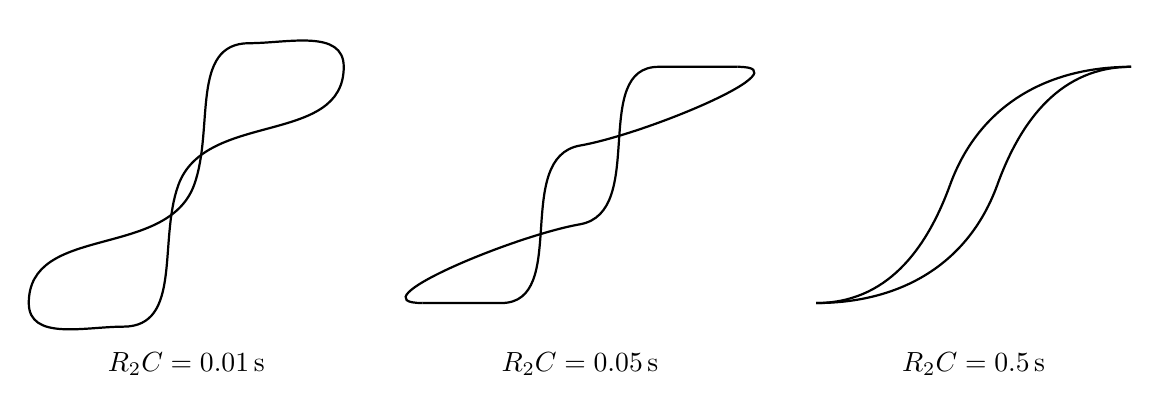
\begin{tikzpicture}
			\draw [thick] (-2,-1.5) to[out=90,in=250] (0.1,0) to[out=70,in=180] (0.8,1.8) to[out=0,in=90] (2,1.5);
			\draw [thick] (-2,-1.5) to[out=270,in=180] (-0.8,-1.8) to[out=0,in=250] (-0.1,0) to[out=70,in=270] (2,1.5);
			\node [below] at(0,-2) {$ R_2C=0.01\,\mathrm s $};
			
			\draw [thick] (3,-1.5) to[out=180,in=190] (5,-0.5) to[out=10,in=180] (6,1.5) to[out=0,in=180] (7,1.5);
			\draw [thick] (3,-1.5) to[out=0,in=180] (4,-1.5) to[out=0,in=190] (5,0.5) to[out=10,in=0] (7,1.5);
			\node [below] at(5,-2) {$ R_2C=0.05\,\mathrm s $};
			
			\draw [thick] (9.7,0) to [out=70,in=180] (12,1.5);
			\draw [thick] (9.7,0) to [out=250,in=0] (8,-1.5);
			\draw [thick] (8,-1.5) to [out=0,in=250] (10.3,0);
			\draw [thick] (10.3,0) to [out=70,in=180] (12,1.5);
			\node [below] at(10,-2) {$ R_2C=0.5\,\mathrm s $};
		\end{tikzpicture}
		\caption{\small 不同积分常量下的李萨如图形}
		\label{fig4}
	\end{figure}
	
	\subsection{实验二:测量样品1的动态磁滞回线}
	(1)根据原始数据计算得到$ H,B $数据如下
	
	\begin{table}[!h]
		\centering
		\begin{tabular}{|c|c|c|c|}
			\hline
			$ \quad H(\mathrm{A/m})\quad $ & $ \qquad B(\mathrm T)\qquad $ & $ \quad H(\mathrm{A/m})\quad $ & $ \qquad B(\mathrm T)\qquad $\\
			\hline
			8.08 & 0.10 & 35.77 & 0.41\\			
			\hline
			10.38 & 0.14 & 39.23 & 0.42\\
			\hline
			13.85 & 0.16 & 42.49 & 0.43\\
			\hline
			16.15 & 0.22 & 45.00 & 0.44\\
			\hline
			18.46 & 0.24 & 47.31 & 0.45\\
			\hline
			21.92 & 0.29 & 50.31 & 0.457\\
			\hline
			24.23 & 0.31 & 53.08 & 0.462\\
			\hline
			26.54 & 0.33 & 70.38 & 0.49\\
			\hline
			30.00 & 0.37 & 20.31 & 0.28\\
			\hline
			32.30 & 0.39 & 28.15 & 0.36\\
			\hline
		\end{tabular}
		\caption{\small 样品1的动态磁化曲线测绘数据表}
		\label{tab3}
	\end{table}
	
	根据上表可绘制动态磁化曲线图如图\ref{fig5}。
	
	(2)根据表\ref{tab3}中数据,可计算得到表\ref{tab4}中数据,进而绘制图\ref{fig6}:
	
	\begin{table}[h]
		\centering
		\begin{tabular}{|c|c|c|c|}
			\hline
			$ \qquad H(\mathrm{A/m})\qquad $ & $ \quad\mu_m(\mathrm{A\cdot T\cdot m/N})\quad $ & $ \qquad H(\mathrm{A/m})\qquad $ & $ \quad\mu_m(\mathrm{A\cdot T\cdot m/N})\quad $\\
			\hline
			8.08 & 9848.7 & 35.77 & 9121.3\\			
			\hline
			10.38 & 10733.0 & 39.23 & 8519.6\\
			\hline
			13.85 & 9193.1 & 42.49 & 8053.3\\
			\hline
			16.15 & 10840.3 & 45.00 & 7780.9\\
			\hline
			18.46 & 10345.9 & 47.31 & 7569.2\\
			\hline
			21.92 & 10528.0 & 50.31 & 7228.6\\
			\hline
			24.23 & 10181.2 & 53.08 & 6926.3\\
			\hline
			26.54 & 9894.7 & 70.38 & 5540.3\\
			\hline
			30.00 & 9814.6 & 20.31 & 10970.8\\
			\hline
			32.30 & 9608.4 & 28.15 & 10176.9\\
			\hline
		\end{tabular}
		\caption{\small 样品1的$ \mu_m-H_m $数据表}
		\label{tab4}
	\end{table}
	
	
	\newgeometry{a4paper,centering,top=-1cm,bottom=2cm,left=0cm,right=0cm}
	\begin{figure}[p]
		\centering
		\includegraphics[]{exp-08.pdf}
		\captionsetup{skip=-40pt}
		\caption{\small $ f=100\,\mathrm{Hz} $下锰锌铁氧体的动态磁化曲线}
		\label{fig5}
	\end{figure}
	\restoregeometry
	
	\newgeometry{a4paper,centering,top=-1cm,bottom=2cm,left=0cm,right=0cm}
	\begin{figure}[p]
		\centering
		\includegraphics[]{exp-08.pdf}
		\captionsetup{skip=-40pt}
		\caption{\small 样品1的$ \mu_m-H_m $曲线}
		\label{fig6}
	\end{figure}
	\restoregeometry

	(3)取表\ref{tab3}前6个数据点进行线性拟合如图\ref{fig7}
	
	\begin{figure}[h]
		\centering
		\includegraphics[scale=1.1]{fig7.png}
		\caption{\small 可逆磁化阶段的$ B-H $的线性拟合}
		\label{fig7}
	\end{figure}

	得到线性拟合函数的斜率$ \dfrac BH $后,将其代入$ \mu_i=\lim\limits_{H\to 0}\dfrac{B}{\mu_0 H} $可计算得到
	\[\mu_i=10743.0\,\mathrm{A\cdot T\cdot m/N}\]
	
	\subsection{实验三:观察不同频率下样品2的动态磁滞回线}
	对原始数据进行运算后可得到所求的$ B_m,B_r,H_C $,即有表\ref{tab5}。
	
	\begin{table}[!h]
		\centering
		\begin{tabular}{|c|c|c|c|}
			\hline
			$ \qquad f(\mathrm{Hz})\qquad $ & $ \qquad B_m(\mathrm T)\qquad $ & $ \qquad B_r(\mathrm T)\qquad $ & $ \quad H_C(\mathrm{A/m})\quad $\\
			\hline
			20 & 0.978 & 0.644 & 120.0\\
			\hline
			40 & 0.978 & 0.622 & 112.0\\
			\hline
			60 & 0.978 & 0.644 & 144.0\\
			\hline
		\end{tabular}
		\caption{\small 不同频率下样品2部分磁化性质参数}
		\label{tab5}
	\end{table}

	表\ref{tab2}与表\ref{tab5}中随着频率的增大,$ B_r $均应有一定程度的减小,实际未测得可能是实验过程中二者差距较小,在当时所用示波器纵向缩放倍率下读数未能得到差异。

	\subsection{实验四:测量样品1在直流偏置磁场下的可逆磁导率}
	对原始数据进行运算之后得到表\ref{tab6}中数据,进而可绘制出图\ref{fig8}中$ \mu_R-H $曲线。
		
	\begin{table}[!h]
		\centering
		\begin{tabular}{|c|c|c|c|}
			\hline
			$ \qquad H(\mathrm{A/m})\qquad $ & $ \quad\mu_R(\mathrm{A\cdot T\cdot m/N})\quad $ & $ \qquad H(\mathrm{A/m})\qquad $ & $ \quad\mu_R(\mathrm{A\cdot T\cdot m/N})\quad $\\
			\hline
			11.54 & 7356.50 & 69.23 & 843.06\\			
			\hline
			23.08 & 5424.14 & 80.77 & 621.51\\
			\hline
			34.62 & 3262.96 & 92.31 & 438.50\\
			\hline
			46.15 & 1779.80 & 103.85 & 377.53\\
			\hline
			57.69 & 1186.53 & 115.38 & 213.58\\
			\hline
		\end{tabular}
		\caption{\small 直流偏置磁场$ H $与$ \mu_R $数据记录}
		\label{tab6}
	\end{table}
	
	\newgeometry{a4paper,centering,top=-1cm,bottom=2cm,left=0cm,right=0cm}
	\begin{figure}[p]
		\centering
		\includegraphics[]{exp-08.pdf}
		\captionsetup{skip=-40pt}
		\caption{\small $ \mu_R-H $曲线}
		\label{fig8}
	\end{figure}
	\restoregeometry

	\section{实验总结}
	\subsection{思考题}
	
	\noindent 1.铁磁材料的动态磁滞回线与静态磁滞回线在概念上有什么区别?铁磁材料动态磁滞回线的形状和面积受哪些因素影响?
	
	\textit{动态磁滞回线是指铁磁材料在交变磁场作用下得到的一条闭合$ B-H $曲线,其特点在于使材料磁化的磁场是交变的,且通常不只有一个周期。}
	
	\textit{静态磁滞回线是指铁磁材料在磁化完全后$ B-H $曲线,实际测量时会选择在磁场强度$ H $的一个周期内缓慢变化其值,测定此时的$ B $,进而绘制得到可近似为静态磁滞回线的准静态磁滞回线。}
	
	\textit{这两种外部条件使得对于静态磁滞回线而言,一次循环磁化过程中的能量损耗(这于$ B-H $曲线所包围的面积成正比)仅包括磁滞损耗;而对于动态磁滞回线,一次循环磁化过程中的能量损耗除了磁滞损耗,还包括涡流损耗。}
	
	\textit{铁磁材料动态磁滞回线的形状和面积和材料本身性质、外磁场的频率与幅度均有关联。}
	
	\textit{材料本身的矫顽力越小,磁滞回线的形状越窄;一般地,交变外磁场的频率越大、幅度越小,磁滞回线所包围的面积越小(饱和后则基本不变);根据涡流损耗$ W=\dfrac{U^2}{R}\cdot t $,电阻率较低材料的磁滞回线所包围的面积越大。}
	
	~\
	
	\noindent 2.铁氧体和硅钢材料的动态磁化特性各有什么特点?
	
	\textit{铁氧体是硬磁材料,硅钢是软磁材料。硬磁材料具有较高的磁导率,相比软磁材料更易被磁化,而软磁材料的矫顽力小,磁滞损耗小。故而铁氧体的动态磁滞回线包围的面积比硅钢更大。}
	
	~\
	
	\noindent 3.本实验中,电路参量应怎样设置才能保证$ u_{R_1}-u_C $所形成的李萨如图形正确反映材料动态磁滞回线的形状?
	
	\textit{由实验原理可知,要使李萨如图形正确反应材料动态磁滞回线形状的条件为使得$\displaystyle B\propto u_C\approx\frac{1}{CR_2}\int u_2\dif t $,即要使$ u_C\ll u_2 $,从而需要设置积分电路中的$ R_2C\gg T $。}
	\subsection{心得体会与反思收获}
	本次实验使用磁特性综合测量实验仪与数字化直流电源,大大简化了电路的搭建与参数调整工作。由此,实验的主要操作在于预科实验中已经学习过的各种示波器操作。在这次实验中,虽然我正确地利用示波器完成了大部分实验数据的读取,但显然表\ref{tab2}\,和表\ref{tab5}\,中$ B_r $值的测量不够精确,可以看出在示波器使用上还有不足。此外实际实验过程中我还曾因未注意到实验所需参数而被迫返工,这样的粗心在以后的实验中应当力求避免。
\end{document}